


In Sec.~\ref{subsec:beampol}, we reviewed in general terms the importance of the
 use of beam polarisation to meet the physics goals of the ILC.  An aspect that we did not stress there is the use of beam 
polarization to control and minimize systematic errors.  Uncontrolled systematic errors can potentially poison any campaign 
of precision measurements.   For the studies of the Higgs boson in which we wish to claim that precisely measured deviations from the SM can give a discovery of new physics, we must be certain that systematic errors are both small and well-constrained. 


\subsubsection{Control of systematic uncertainties using beam polarisation} 
\label{subsubsec:pol:systematics}

Before summarising the possible sources of systematic error in our Higgs coupling measurements, we review the use of beam polarization
in controlling these  uncertainties. A general statement is that it is important to measure effects correlated to systematic uncertainties.  For this, it is crucial to always have one more degree of freedom that (statistically) absolutely required: For physics measurements which do not aim at the analysis of a chiral structure, e.g.\ measurements of total unpolarised cross sections, two data sets with with different polarisations (e.g.\ $\Pmp=(\pm 80\%, \mp 30\%)$ or $\Pmp=(\pm 80\%, 0)$ often suffice to constrain the most important nuisance parameters. However if the chiral structure itself is among the observables, e.g.\ when measuring \ALR\ of 2-fermion processes or of Higgsstrahlung, one flip of the polarisation sign(s) is already contained in the observable itself, and thus a non-zero positron polarisation becomes essential to provide enough independent information to constrain nuisance parameters.

The evaluation of systematic uncertainties for experiments which have not yet been built is a difficult task and will to some extent always remain guess-work until real data have been taken. Important is therefore to include the experience from previous $e^+e^-$ experiments, especially at LEP, where many uncertainties could be controled to a typical level of 1\%. Assuming that the same level can be reached at future $e^+e^-$ colliders, detailed studies of systematic uncertainties at the ILC have concentrated on cases where the statistical uncertainties are expected to be significantly below 1\%, and on searches in channels with large irreducible backgrounds. An example for the first case is a global analysis of total rates and differential distributions of various 2-fermion and 4-fermion SM processes, extracting simultaneously the total unpolarised cross sections, the relevant left-right asymmetries, the beam polariations and the charged triple gauge couplings, see Sec.~\ref{subsec:ew_WWana} and Ref.~\cite{bib:PhDRobert}. An example for the second category is the WIMP search in the mono-photon channel, see Sec.~\ref{sec:searches} and Ref.~\cite{Habermehl:417605}. 

In the remainder of this section we will highlight the relative impact of the beam polarisation on the control of systematic uncertainties using these two studies as examples. The consequences for the treatment of systematic uncertainties in the Higgs coupling fit will be discussed in the next subsection.

\begin{itemize}
\item {\textbf{Fast-helicity reversal and correlations between data sets:}} The design of the ILC includes the capability to flip the sign of the two beam polarisations independently and on a train-by-train basis, as introduced in Sec.~\ref{par:beampol}. This helicity reversal is fast compared to typical time-scales of changes in the configuration, calibration and alignment of the detector and the accelerator, and thus data sets with the same beam energy but different beam helicities can be considered as being collected ``quasi-concurrently''. Therefore, many of the experimental systematic effects will be correlated to a large degree between data sets with different polarisations. Note that this does not apply for data sets with different center-of-mass energies, which are collected after each other, typically in different years, and thus systematic effects can in general not be expected to be correlated between such data sets.
Similarly, also most theoretical uncertainties will be correlated between same-energy-different-polarisation data sets, apart from those which directly concern the dependence of the polarised cross sections on the beam polarisations, so effectively any uncertainty to Eqn.~\ref{eq:pol:xsec} {\color{red} [JL: I can't think of any uncertainty to this very basic relation, but I don't dare to say that there is none - comments welcome!]}.  

As example, Fig.~\ref{fig:alpha_error_corr_uncorr} shows the uncertainties $\Delta \alpha $ on the unpolarised cross sections of various 2-fermion and 4-fermion processes as obtained from the global fit introduced above~\cite{bib:PhDRobert}, for the example of a 1\% uncertainty on selection efficiencies and purities, each. In the pesence of beam polarisation, it is assumed that only 10\%, thus 0.1\%, remain uncorrelated between the data sets of different polarisations. In absence of beam polarisation, there are no data sets with correlated systematic uncertainties, and the impact on the cross section uncertainties increases by a factor of 2 for $WW$ and single-$W$ processes, and a factor of 5 for $s$-channel $Z/\gamma$ exchange.
\begin{figure}
\centering
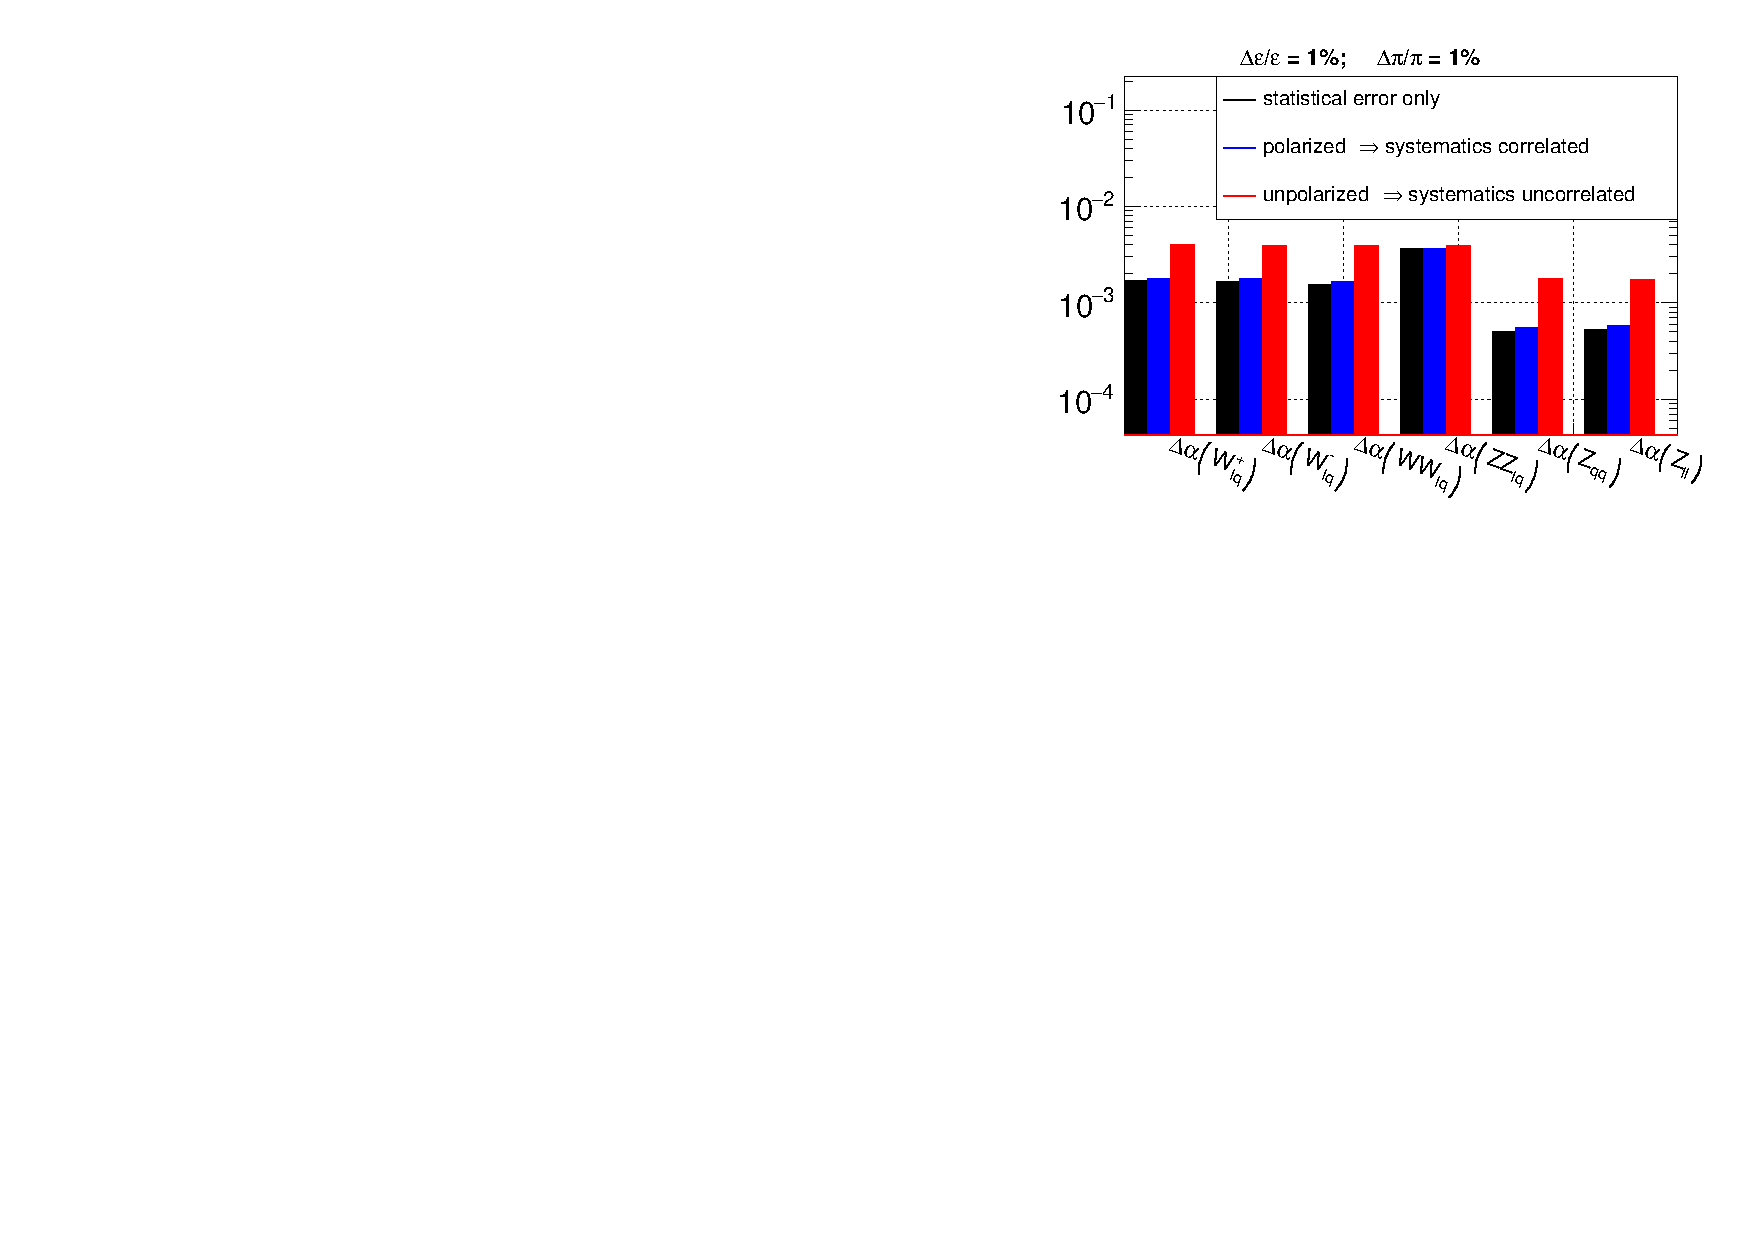
\includegraphics[width=0.95\linewidth]{./chapters/figures/ElectroWeakSysDependency_alpha_short.pdf}
		
\caption{Uncertainties on the unpolarised cross sections of various 2-fermion and 4-fermion processes as obtained from the global fit introduced in the text~\cite{bib:PhDRobert}, assuming a systematic uncertainty of 1\% on the selection efficiencies and purities, each. In the case of polarised beams, it is assumed that only 10\% of the uncertainty is uncorrelated between data sets - in this case the impact of the systematic uncertainties is minimal. Without the redundancies provided by data sets with correlated systematic uncertainties, the total uncertainties increase by a factor 2 for $WW$ and single-$W$ processes and a factor of 5 for 2-fermion processes.}
\label{fig:alpha_error_corr_uncorr}
\end{figure}

Note that this example so far only considers normalisation uncertainties. When adding shape uncertainties, however, the benefit from the redundacy offered by several data sets with correlated systematic effects is expected to be even more pronounced than in the current case of only normalisation uncertainties, since the shape uncertainties will reduce the information which can be extracted from the  differential distributions included in the fit.  

\item {\textbf{Impact of positron polarisation on \ALR\ measurement:}} The left-right asymmetries \ALR\ themselves are obviously only accessible when at least electron beam polarisation is available. Still the positron polarisation is crucial in order to reach ultimate precision on \ALR, as illustrated in Fig.~\ref{fig:beta_error_noposipol}, again from the global fit to 2- and 4-fermion processes. In this example, no detector or theory systematics are included, only the exact polarisation values are treated as nuisance parameters. It can be seen that in the absence of positron polarisation, the uncertainties on \ALR\ increase by 2 factor 2 on $WW$ production and by a factor of $10$ on $s$-channel $Z$ exchange. only the single-$W$ processes remain unaffected.


\begin{figure}
\centering
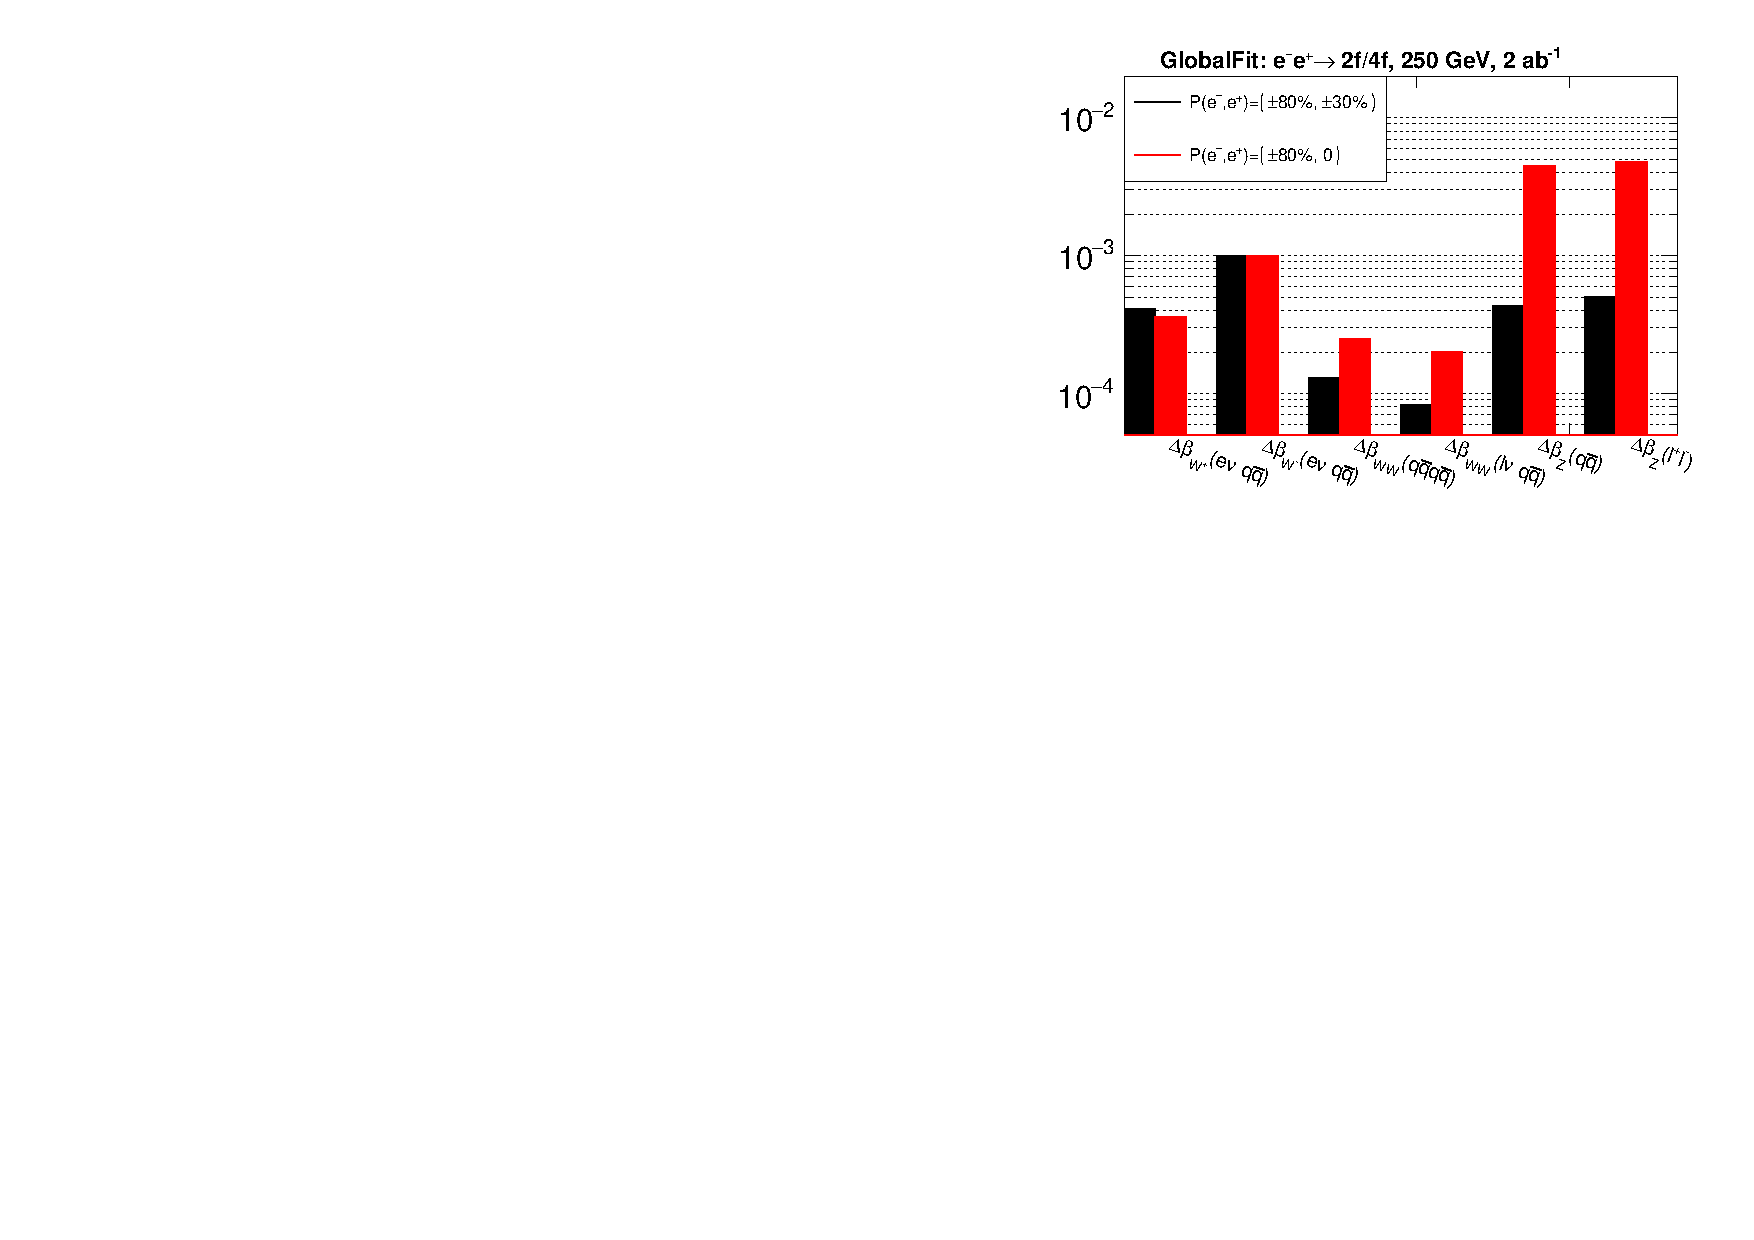
\includegraphics[width=0.95\linewidth]{./chapters/figures/beta_precision_upolarized.pdf}
		
\caption{Uncertainties $\Delta \beta$ on \ALR\ of various 2-fermion and 4-fermion processes as obtained from the global fit introduced in the text~\cite{bib:PhDRobert} with both beams polarised (with the standard 45\%/45\%/5\%/5\% sharing between the four helicity configurations) and in the absence of positron polarisation (with a 50\%/50\% sharing between the two remaining helicity configurations). In the absence of positron polarisation, the  uncertainties on \ALR\ increase by a factor 2 for $WW$ and by about a factor of 10 for 2-fermion processes. Alone the single-$W$ processes remain unaffected.}
\label{fig:beta_error_noposipol}
\end{figure}

\item{\textbf{Undetected biases:}} When considering the level of precision the ILC is aiming for, and even more so when attempting to go even further, even subtle biases can propagate to the results when not treated properly. As example, let's consider the case of operation with an unpolarised positron. In this case, one could assume that it would be fully sufficient to fix the nuisance parameters for the positron polarisation to zero. However it has been shown in~\cite{bib:PhDRobert} that in this case even a residual positron polarisation at the permille-level would already create a noticible bias on cross sections and asymmetries of the same order  of magnitude. This would make it hard to decide whether any possibly observed discrepancy from the SM expectation is a hint for new physics or due to a systematic effect. Therefore for ultimate precision, both beam polarisations should be treated as nuisance parameters independently of their absolute size.

\item {\textbf{Shape uncertainties and beam polarization:}} Uncertainties on the shape of distributions have been included in the WIMP search in the mono-photon channel~\cite{Habermehl:417605}. Figure~\ref{fig:polWIMPsys} shows the expected exclusion limit on the new physics scale $\Lambda$ as function of the WIMP mass for the same study cases as Fig.~\ref{fig:polWIMPstat}. The study includes a careful evaluation of the systematic uncertainties, comprising those on selection efficiencies, luminosity, beam energy (spectrum) and polarization as well as on the theoretical modelling of the background. 
The limit calculation uses a fractional event counting based on the observed energy spectrum of the selected photon candidates and considers normalisation and shape-dependent uncertainties as well as their (partial) correpations. The signal strength thereby has to be constrained on top of a significant irreducible background from $e^+e^- \to \nu\bar{\nu}\gamma$ and radiative low-angle Bhabha scattering. For increasing WIMP masses, the maximum possible energy of the ISR photons becomes lower. For the highest WIMP masses, the signal-free part of the spectrum becomes sufficiently large to constrain the nuisance parameters and thus to limited the impact of the systematic uncertainties. This effect is visible in form of the ``bump'' in the limit curves near $M_X=220$\,GeV. In case of the unpolarised data set, the effect starts to become visible already from $M_X=150$\,GeV onwards,
but the exclusion remains much weaker than in the polarised case. Comparison with Fig.~\ref{fig:polWIMPstat} shows that the benefit of polarisation in presence of systematic uncertainties goes significantly beyond the purely statistical $S/B$ effect. In particular it should be noted that when the systematic effects are included, the splitting of the total luminosity into four different data sets allows to set more stringent limits as if all luminosity would just be dedicated to the ``statistically-prefered'' helicity combination. In fact the result for only one helicity combination suffers as much from the systematic uncertainties as the unpolarised case, while in case of the polarisation mix, when four data sets with different helicities are used, the sensitivity is only affected veru weakly by the systematic uncertainties.



\begin{figure}
\centering
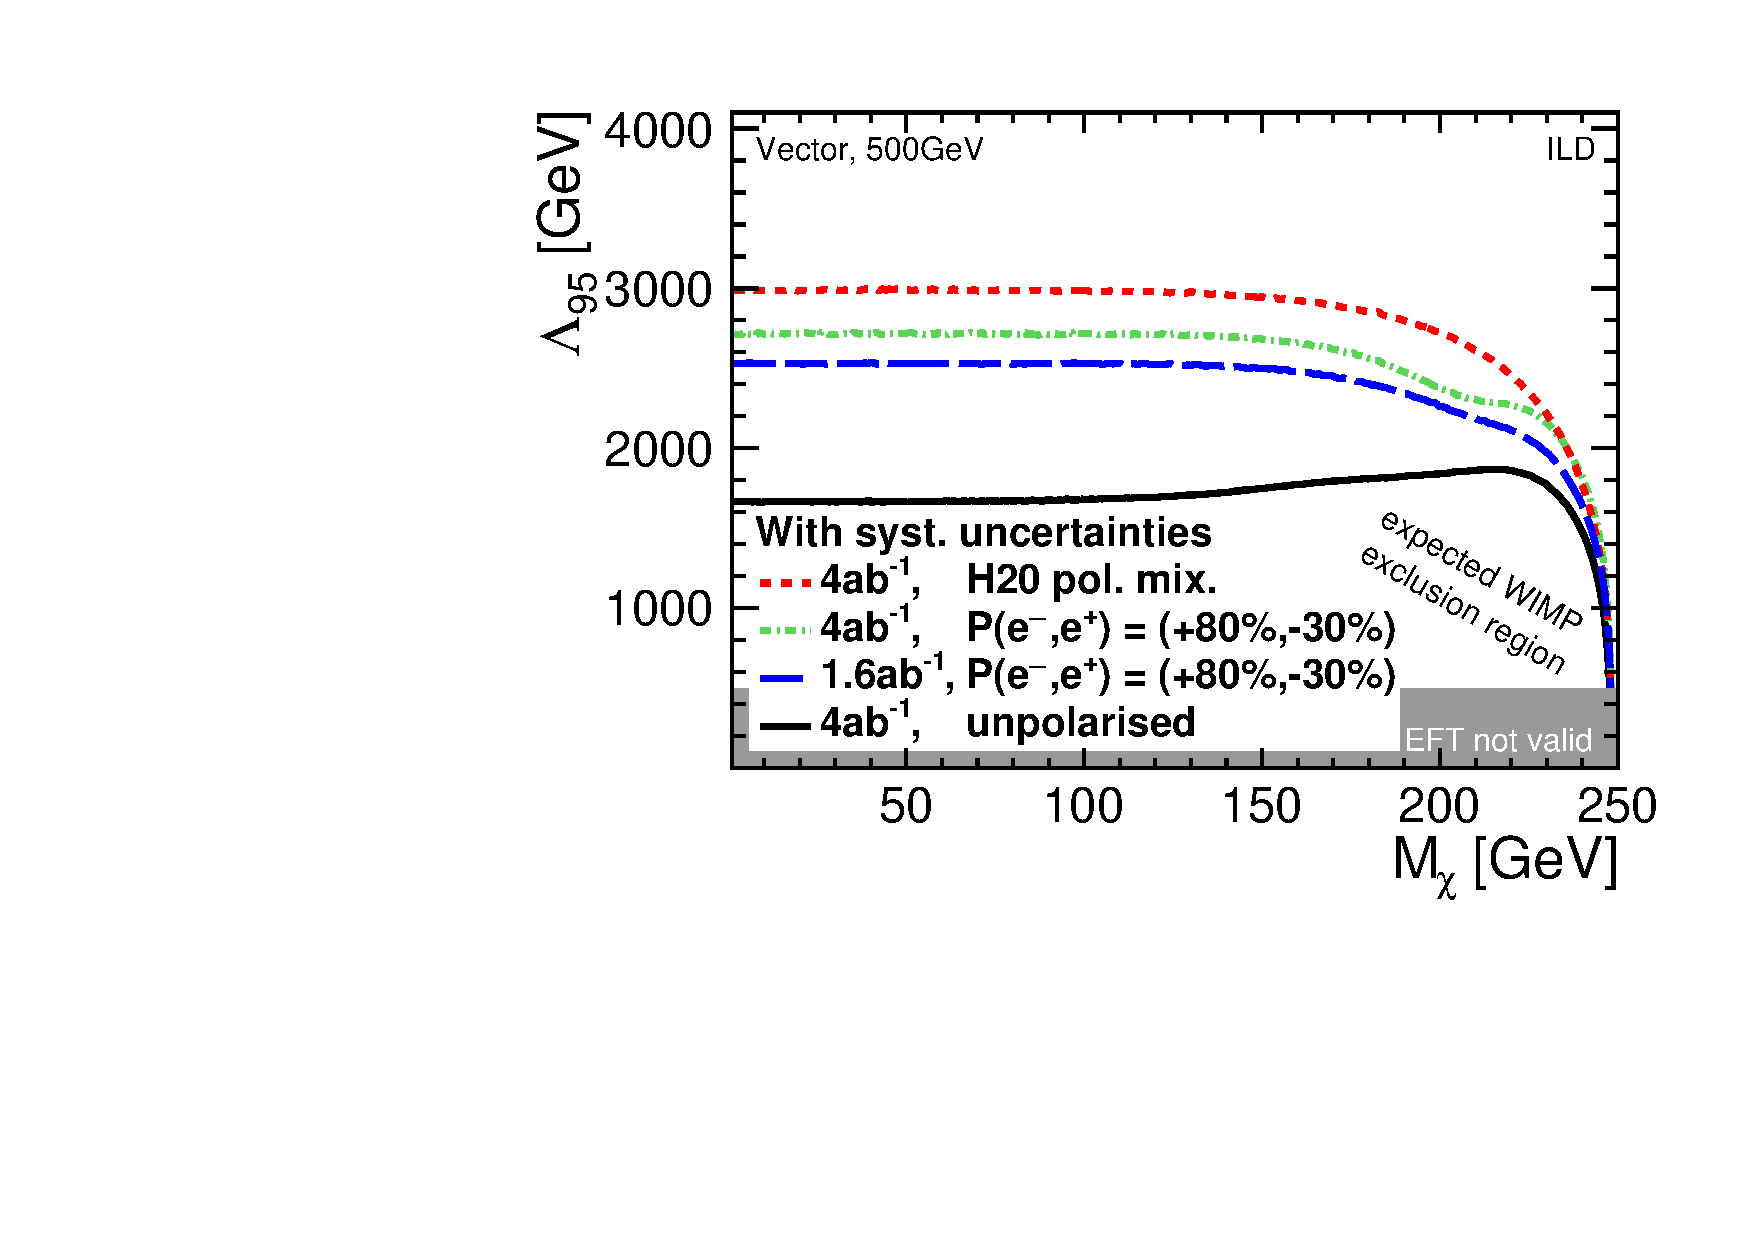
\includegraphics[width=0.95\linewidth]{./chapters/figures/vector_withSystematics.pdf}
		
\caption{Comparison of the reach of the search for WIMP production in the mono-photon channel for different assumptions on luminosity and polarization, {\em including} systematic uncertainties (see Sec.~\ref{sec:searches} for a description of the analysis)~\cite{Habermehl:417605}. }
\label{fig:polWIMPsys}
\end{figure}

\end{itemize}

\subsubsection{Systematic uncertainties considered in the Higgs coupling fit}
The Higgs coupling fits discussed in the following sections include the following systematic uncertainties:
\begin{itemize}
\item The luminosity at the ILC will be measured from low-angle Bhabha scattering with the help of a dedicated forward calorimeters, the LumiCals (see Sec.~\ref{sec:detectors} and Ref.~\cite{Abramowicz:2010bg}). This measurement is extremely sensitive to the exact alignment of the LumiCals on the two sides of the detector, as well as to beam backgrounds and has been studied in detailed simulations both for the ILC and for CLIC~\cite{Bozovic-Jelisavcic:2014aza, Lukic:2013fw}. Based on these studies, the resulting systematic uncertainty on all Higgs cross section and cross-section-times-braching-ratio measurements is assumed to be 0.1\%
\item Another 0.1\% is assumed for the net systematic effect of the finite knowledge of luminosity-weighted long-term average values of the beam polarisations at the $e^+e^-$ interaction point. While the Compton polarimeters in the Beam Delivery System resolve time-dependencies at the level of 0.25\%~\cite{Vormwald:2015hla, List:2015lsa}, also the effects of spin transport, misalignment of beam line magnets as well as depolarisation during the beam-beam interaction have been studied~\cite{Beckmann:2014mka}. The absolute scale of the luminosity-weighted average polarisation at the IP is finally calibrated from collision data, e.g.\ a global fit SM processes with a strong polarisation dependence~\cite{bib:PhDRobert}. 
\item Theoretical uncertainties are also assumed to have reched at the level of 0.1\% by the time of ILC operation {\color{red}[Any good \textbf{theoretical} arguments to add here?]}. This number is justified in case of polarised beams by the global fit study discussed above~\cite{bib:PhDRobert}, which showed that the absolute normalisations of cross sections and left-right asymetries can be controled  at this level. In the case of unpolarised beams, the theoretical uncertainties would require a much more detailed consideration.
\item As mentioned already at the beginning of Sec.~\ref{subsubsec:pol:systematics} experimental systematics on selection efficiencies, flavour tagging, detector calibrations etc of 1\% have already been reached at LEP in many cases. With the advances in detector technology and the larger integrated luminosity, we assume that for each data set at the ILC this can be reduced by a factor of 3 to 0.3\%. These 0.3\% are considered as net effect of all experimental uncertainties in the absence of beam polarisation.

In the presence of both beam polarisations, the net effect of systematic uncertainties has been shown to be smaller by factors between 2 and 10 due to the correlations between data sets with different beam polarisations as discussed in Sec.~\ref{subsubsec:pol:systematics}. Since the Higgs coupling fit does not yet comprise such a detailed treatment of systematic uncertainties and their correlations as the above mentioned global fit to 2-fermion and 4-fermion processes, we assume that, in presence of polarised beams, the net effect of the experimental uncertainties reduces to 0.1\%.
\end{itemize}




